
\documentclass[12pt]{amsart}

\usepackage[utf8]{inputenc}
\usepackage[T1]{fontenc}
\usepackage{lmodern}
\usepackage[ngerman]{babel}
\usepackage{graphicx}
\usepackage{paralist}

\usepackage{Macros}

% No indent at begin of paragraph
\setlength{\parindent}{0pt}
% line break after subsubsection heading
\makeatletter
\def\subsubsection{\@startsection{subsubsection}{3}%
  \z@{.5\linespacing\@plus.7\linespacing}{.1\linespacing}%
    {\normalfont\itshape}}
    \makeatother

\usepackage{geometry} % see geometry.pdf on how to lay out the page. There's lots.
\geometry{a4paper} % or letter or a5paper or ... etc
% \geometry{landscape} % rotated page geometry

\title{Hausaufgabe 3 - Blatt 8, 9 \& 10}
\author{Sarah Köhler und Matthias Loibl}
\date{} % delete this line to display the current date

%%% BEGIN DOCUMENT
\begin{document}

\maketitle
%\tableofcontents

%\section*{Blatt 8}
\section*{Aufgabe 1: Verbände}
\subsection*{a)}

\begin{figure}[h!]
\begin{center}
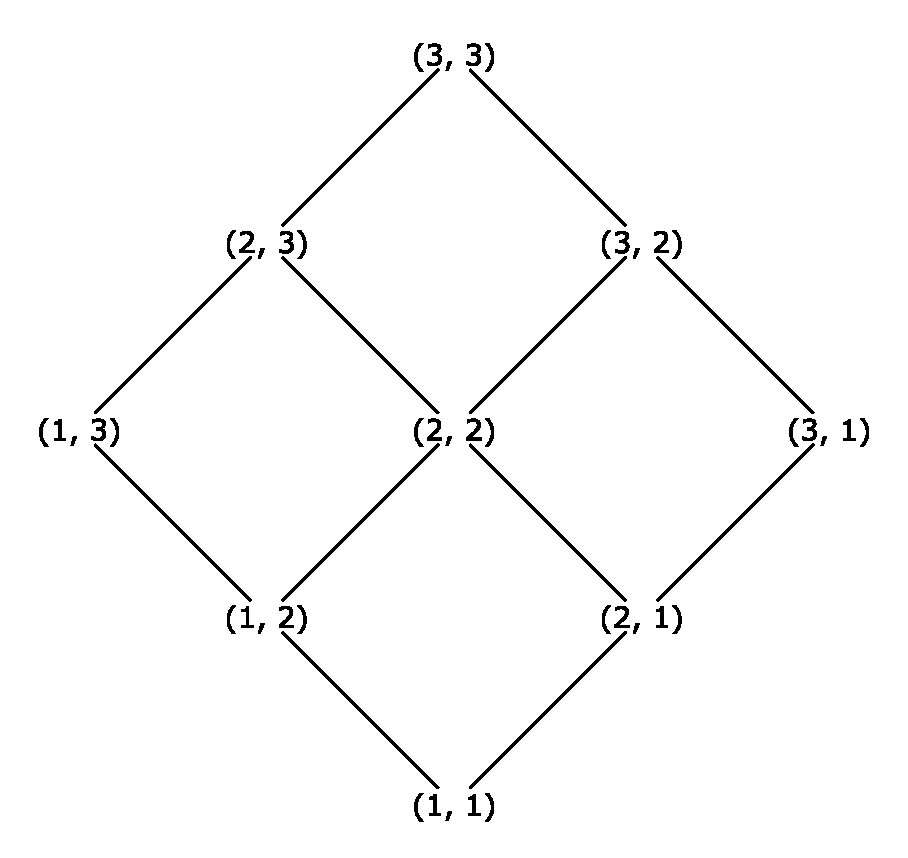
\includegraphics[width=13cm]{aufgabe1a-hasse}
%\caption{This is a figure.}
\end{center}
\end{figure}

\subsection*{b)}
Gegeben zwei Elemente $(x_1, y_1) \in \mathbb{N}^+ \times \mathbb{N}^+ $ und
$(x_2, y_2) \in \mathbb{N}^+ \times \mathbb{N}^+ $ kann das Infimum mit folgender Funktion berechnet werden:

\begin{align*}
&inf:  (\mathbb{N}^+ \times \mathbb{N}^+) \times  (\mathbb{N}^+ \times \mathbb{N}^+)  \to \mathbb{N}^+ \times \mathbb{N}^+ \\
&((x_1, y_1), (x_2, y_2))  \mapsto (min(x_1, x_2), min(y_1, y_2))
\end{align*}

Das Supremum berechnet diese Funktion:
\begin{align*}
&sup:  (\mathbb{N}^+ \times \mathbb{N}^+) \times  (\mathbb{N}^+ \times \mathbb{N}^+)  \to \mathbb{N}^+ \times \mathbb{N}^+ \\
&((x_1, y_1), (x_2, y_2))  \mapsto (max(x_1, x_2), max(y_1, y_2))
\end{align*}

\subsection*{c)}
Sei $ X \subseteq  \mathbb{N}^+ \times \mathbb{N}^+ $ und $ x \in X$. Dann lässt sich das Infimum mit folgender Funktion berechnen:
\begin{align*}
& \Inf : X \to x \\
& \Inf (X) = (min(\{x \medspace | \medspace \exists y. (x, y) \in X\}),
min(\{y \medspace| \medspace\exists x. (x, y) \in X\})
% TODO: abstände um | schöner machen
\end{align*}

Das Supremum berechnet diese Funktion:
\begin{align*}
& \Sup : X \to x \\
& \Sup (X) = (max(\{x \medspace| \medspace\exists y. (x, y) \in X\}),
max(\{y \medspace| \medspace\exists x. (x, y) \in X\})
% TODO: Abstände
\end{align*}
Für unendliche Teilmengen $X$ ist die Funktion undefiniert, da dann $max$ kein größtes Element finden kann.

\subsection*{d)}

\begin{align*}
& \bot = (0, 0)
\end{align*}
$\top $ existiert nicht, da die Trägermenge $ \mathbb{N}^+ \times \mathbb{N}^+ $ das Kreuzprodukt der natürlichen Zahlen ist.
Da $\mathbb{N} $ unendlich ist und kein größtes Element besitzt, gibt es auch in $ \mathbb{N}^+ \times \mathbb{N}^+ $ kein größtes Element.

\subsection*{e)}
$V$ ist ein Verband, da die Funktionen aus Aufgabenteil b) für jede zweielementige
 Teilmenge von $V$ das Infimum und das Supremum berechnen können.
Allerdings ist $V$ kein vollständiger Verband, da die Funktion $\Sup$ aus
Aufgabenteil c) für unendliche Teilmengen der Trägermenge undefiniert ist.
Das heißt es existiert nicht für alle Teilmengen der Trägermenge von $V$
 ein Supremum und somit kann $V$ kein vollständiger Verband sein.

\subsection*{f)}
Zu zeigen: Für alle $(x_1, y_1), (x_2, y_2) \in \mathbb{N}^+ \times \mathbb{N}^+ $ gilt: \\
$ (x_1, y_1) \leq_2 (x_2, y_2) \Rightarrow f((x_1, y_1)) \leq_2 f((x_2, y_2))$ \\
Seien $g$ und $h$ Funktionen: \\

\begin{align*}
& g: \mathbb{N}^+ \to  \mathbb{N}^+\\
&  g(x) = x! \\
& h: \mathbb{N}^+ \to  \mathbb{N}^+\\
&  h(y) = 2y^2 +2y -1 \\
\end{align*}
Es gilt offensichtlich:
\begin{align*}
& f((x, y)) = (h(y), g(x))
\end{align*}
Seien $ (x_1, y_1), (x_2, y_2) \in \mathbb{N}^+ \times \mathbb{N}^+ $
 mit $ (x_1, y_1) \leq_2 (x_2, y_2) $.
Dann gilt:

\begin{align}
& f((x_1, y_1)) = (h(y_1), g(x_1))
\end{align}

Es gilt außerdem:

\begin{align}
& f((x_2, y_2)) = (h(y_2), g(x_2))
\end{align}

Um die Prämisse zu erfüllen muss gelten:
\begin{align*}
& f((x_1, y_1)) \leq_2 f((x_2, y_2)) \\
\end{align*}
Aus (1) und (2) folgt, das folgendes ebenso gelten muss \\
\begin{align*}
& \Leftrightarrow (h(y_1), g(x_1)) \leq_2 (h(y_2), g(x_2)) \\
\end{align*}
Aus der Definition von  $\leq_2 $ folgt, dass dazu gelten muss: \\
\begin{align*}
& \Leftrightarrow h(y_1) \leq h(y_2) \land  g(x_1) \leq g(x_2) \\
\end{align*}

Betrachte beide Voraussetzungen getrennt: \\
1. Zu zeigen: $ h(y_1) \leq h(y_2) $ \\
Das gilt mit $y_1 \leq y_2$ immer, wenn $h$ monoton ist. \\
Dazu muss gelten: $h(n) \leq h (n+1), n \in \mathbb{N}^+$ \\
\begin{align*}
 h(n) &= 2n^2+2n-1 &\\
&\leq 2n^2 +6n +3 = 2n^2 +4n +2 +2n +2 -1 & n > 0\\
& = 2(n+1)^2 + 2(n+1) -1 = h(n+1) &\\
\end{align*}
Also ist $h$ monoton und die erste Voraussetzung gilt.

2. Zu zeigen: $g(x_1) \leq g(x_2) $ \\
Das gilt unter der gegebenen Voraussetzung $ x_1 \leq x_2 $ immer,
wenn $g$ monoton ist. \\
Dazu muss gelten: $g(n) \leq g(n+1), n \in \mathbb{N}^+ $ \\
\begin{align*}
g(n) &= n! &\\
&\leq (n+1) * n! & n > 0\\
& =(n+1)!= g(n+1)&
\end{align*}
Also ist auch $g$ monoton und die zweite Voraussetzung gilt ebenso.\\

Aus der Gültigkeit beider Voraussetzungen folgt, dass auch $f$ monoton ist.\\
$\Box$



%Das gilt mit $y_1 \leq y_2$ immer, wenn h monoton ist. \\
%Beweis der Monotonie von h per vollständige Induktion:\\
%Induktionsbehauptung: $\forall n \in \mathbb{N}^+. h(n) \leq h(n+1)$ \\
%Induktionsanfang $n = 1$ \\
%$ h(n) = h(1) = 2 + 2 -1 = 3 $\\
%$ h (n +1) = h(2) = 8 + 4 -1 = 11 $\\
%Damit gilt die IB für ein $ n \in \mathbb{N}$.\\
%Induktionsvoraussetzung: Es gilt $h(n) \leq h(n+1)$ \\
%Induktionsschritt: Betrachte $ n+1$ \\
%Zu zeigen: $ h(n+1) \leq h(n+1+1) $\\
%$ h(n+1) = 2(n+1)^2 + 2(n+1) -1 $ \\
%$ = 2(n+1)^2 +2n + 2 -1 = 2(n+1)^2 + 2n + 1 $\\
%$ = 2(n^2 + 2n + 1) + 2n + 1 $ \\
%$ = 2n^2 + 4n + 2+ 2n +1 $ \\
%$ = 2n^2 + 6n +3 $\\
%Mit $ n > 0 $und der IV gilt: \\
%$ \le 2n^2 + 10n + 11 $ \\
%$ = 2n^2 + 8n +8 + 2n + 4 -1 $ \\
%$ = 2(n^2 +4n+4) + 2n +4 -1 $ \\
%$= 2(n+2)^2 + 2(n+2) -1$\\
%$ = h( n + 2) = h(n+1+1)$ \\
%Somit gilt die Induktionsbehautung für ein $ n $ sowie $(n+1)$,
% also für alle $n \in \mathbb{N}^+$.
%
%
%
%2. Zu zeigen: $ g(x_1) \leq g(x_2) $\\
%Das gilt mit $ x_1 \leq x_2$ immer, wenn g monoton ist.\\
%TODO: Beweis der Monotonie von g (vollst. Induktion)
%
%Somit gelten beide Voraussetzungen und damit ist auch f monoton.\\
%$\Box $
 % fertig
\subsection*{Aufgabe 2 - Hennessy-Milner Logik: Formalisierung}

\subsubsection*{a)}

i) 
\begin{align*}
F_1 =& \poss{elefanten}\poss{warte 1min}\poss{warte 1min}\poss{robben}\true\\
\end{align*}

ii) 
\begin{align*}
F_2 =& \poss{robben}\poss{verlassen}\true\\
\end{align*}

iii) 
\begin{align*}
F_3 =& \necess{robben}\necess{verlassen}\false\\
\end{align*}

iv) 
\begin{align*}
F_4 =& \necess{robben}\necess{nilpferde}\false\\
\end{align*}

v) 
\begin{align*}
F_5 =& \poss{jahreskarte}\poss{känguru}\true\\
	&\lor\poss{bezahlen}\poss{kartezeigen}\poss{känguru}\true\\
\end{align*}

\subsubsection*{b)}

\begin{align*}
\denot{F_1}
	=& \{WNK\} 	& ja, da WNK \in \denot{F_1} = \{WNK\}\\
\denot{F_2}
	=& \{WE\} 	& ja, da \denot{F_5} \neq \emptyset\\
\denot{F_3}
	=& \Proc \setminus \{WE\} 	& ja, da \denot{F_5} \neq \emptyset\\
\denot{F_4}
	=& \Proc\\
\denot{F_5}
	=& \{Eingang\}
\end{align*}
 % fertig
\section*{Aufgabe 3: Bisimulation}

\begin{alignat*}{3}
\mathcal{F}^{1}(Proc \times Proc) &= r(s(\{&&(P_1, P_2),(P_1, P_5),(P_1, Q_1), (P_1, Q_2),(P_2, P_5),(P_2, Q_1),\\
								  &		  &&(P_2, Q_2),(P_3, Q_3),(P_4, Q_4),(P_5, Q_2),(P_5, Q_1),(Q_1, Q_2)\}))
\end{alignat*}
\\
$\mathcal{F}^{2}(Proc \times Proc) = r(s(\{(P_1, P_5),(P_1, Q_1),(P_2, Q_2),(P_3, Q_3),(P_5, Q_1)\}))$
\\
$\mathcal{F}^{3}(Proc \times Proc) = r(s(\{(P_2, Q_2),(P_5, Q_1)\}))$
\\
$\mathcal{F}^{4}(Proc \times Proc) = r(s(\{(P_5, Q_1)\}))$
\\
$\mathcal{F}^{5}(Proc \times Proc) = r(s(\{(P_5, Q_1)\}))$
\\\\
Da $\mathcal{F}^{4} = \mathcal{F}^{5}$ sind beide ein Fixpunkt.
\\
Somit erhalten wir, dass $P_5$ und $Q_1$ das einzige nicht trivial bisimilare Paar ist. Es gilt $P_5$ \bisim $Q_1$
 % fertig

%\section*{Blatt 9}
\section*{Aufgabe 4: Bisimulation (2)}

$\mathcal{F}^{1}(Proc \times Proc) = r(s(\{(R_1, R_7),(R_2, R_4),(R_2, R_6),(R_3, R_5),(R_4, R_6),(R_8, R_9)\}))$
\\
$\mathcal{F}^{2}(Proc \times Proc) = r(s(\{(R_2, R_6),(R_3, R_5)\}))$
\\
$\mathcal{F}^{3}(Proc \times Proc) = r(s(\{(R_2, R_6),(R_3, R_5)\})) = \mathcal{F}^{2}$
\\\\
Da $\mathcal{F}^{2} = \mathcal{F}^{3}$ sind beide ein Fixpunkt.
\\
Somit erhalten wir, dass $R_2$ und $R_6$ sowie $R_3$ und $R_5$ die einzigen nicht trivialen bisimilaren Paare sind. Es gilt $R_2$ \bisim $R_6$ und $R_3$ \bisim $R_5$.
 % fertig
\subsection*{Aufgabe 5 - Unterscheidende Formeln}

\subsubsection*{a)}

Es existiert keine unterscheidende Formel, da der Unterschied zwischen den beiden Prozessen nicht durch HML-Formeln beschrieben werden kann.
In $A$ und $B$ ist zu jeder Zeit ein $a$-Schritt möglich. Für beliebige $n \in \mathbb{N}$ sind die beiden Prozesse also n-Schritt-bisimilar: $ A \bisim_n B$. \\
Das Hennessy-Milner-Theorem ist nicht anwendbar, da es voraussetzt, dass beide betrachteten Prozesse bild-endlich sind.
 $A$ ist aber nicht bild-endlich, da die Menge der durch $a$ erreichbaren Nachfolger von $A$ unendlich ist:
$ \#(Der(A,a) \not\in \mathbb{N}$.


\subsubsection*{b)}

Eine unterscheidende Formel ist: \\
$ F_1 = \poss{a}^{11} \true$ \\
Es gilt:
$ B \models F_1$, aber $C \not\models F_1 $.\\


\subsubsection*{c)}

Eine unterscheidende Formel ist: \\
$ F_2 = \poss{a} \necess{a}\false$ \\
Es gilt:
$ Y \models F_2$, aber $X \not\models F_2 $.\\

\subsubsection*{d)}

Es existiert keine unterscheidende Formel, da der Unterschied zwischen den beiden Prozessen nicht durch HML-Formeln beschrieben werden kann.
In $X$ und $Z$ sind zu jeder Zeit $a$-, $\Out{a}{}$- oder $\tau$-Schritte möglich. Für beliebige $n \in \mathbb{N}$ sind die beiden Prozesse also n-Schritt-bisimilar: $ X \bisim_n Z$. \\
Das Hennessy-Milner-Theorem ist nicht anwendbar, da es voraussetzt, dass beide betrachteten Prozesse bild-endlich sind.
 $X$ ist aber nicht bild-endlich, da die Mengen der durch $a, \Out{a}{}$ und $\tau$ erreichbaren Nachfolger von $X$ unendlich sind: \\
$ \#(Der(X,a) \not\in \mathbb{N}$. \\
$ \#(Der(X,\Out{a}{}) \not\in \mathbb{N}$. \\
$ \#(Der(X,\tau) \not\in \mathbb{N}$.
 % fertig
\documentclass[11pt]{paper}

%\usepackage[T1]{fontenc}
\usepackage[utf8]{inputenc}
\usepackage[ngerman]{babel}
%\usepackage[]{}


\begin{document}

\end{document} %

%\section*{Blatt 10}
\subsection*{Aufgabe 7 - Monotonie von O}


Zu zeigen: $\OSem{F}{}$ ist monoton $\forall F \in \henMil_{\{X\}}$. \\
Seien $S_1, S_2 \subseteq \Proc$ und es gelte $S_1 \subseteq S_2$.

Um die Monotonie von $\OSem{F}{}$ für beliebige $F$ zu beweisen, muss also gezeigt werden, dass
 $ \OSem{F}{S_1} \subseteq \OSem{F}{S_2}$ für alle $F \in \henMil$ gilt.

Beweis per struktureller Induktion über den Aufbau von $F$:

\subsubsection*{Induktionsanfang}
Induktionsanfang sind die atomaren Formeln $\true$ und $\false$: \\

\begin{align*}
\OSem{\true}{S_1} =& \Proc \subseteq \Proc  & Def. \OSem{}{}\\
=& \OSem{\true}{S_2} & Def. \OSem{}{}
\end{align*}

\begin{align*}
\OSem{\false}{S_1} =& \Proc \subseteq \Proc & Def. \OSem{}{} \\
=& \OSem{\false}{S_2} & Def. \OSem{}{}
\end{align*}

\subsubsection*{Induktionsvoraussetzung}

Seien $F, G \in \henMil$ so, dass $\OSem{F}{S_1} \subseteq \OSem{F}{S_2}$ und
$\OSem{G}{S_1} \subseteq \OSem{G}{S_2}$ gelten.



\subsubsection*{Induktionsbehauptung I}

Dann gilt auch:
$\OSem{F \lor G}{S_1} \subseteq \OSem{F \lor G}{S_2} $ \\

\subsubsection*{Induktionsschritt I}



\begin{align*}
\OSem{F \lor G}{S_1} =& \OSem{F}{S_1} \cup \OSem{G}{S_1}
 & Def. \OSem{}{}\\
=& \{ p \in \Proc | p \in \OSem{F}{S_1} \lor p \in \OSem{G}{S_1} \}
& Def. \cup \\
\subseteq &  \{ p \in \Proc | p \in \OSem{F}{S_2} \lor p \in \OSem{G}{S_2} \}
& (*) \\
=&  \{ p \in \Proc | p \in \OSem{F}{S_1} \} \cup
  \{ p \in \Proc | p \in \OSem{G}{S_1} \}
& Def. \cup \\
=& \OSem{F}{S_2} \cup \OSem{G}{S_2} & Def. \OSem{}{}\\
=& \OSem{F \lor G}{S_2} &
\end{align*}

$(*)$
Aus der I.V. folgt: \\
\begin{align*}
& p \in \OSem{G}{S_1} \Rightarrow  p \in \OSem{G}{S_2} \\
& p \in \OSem{F}{S_1} \Rightarrow  p \in \OSem{F}{S_2} \\
& \Rightarrow \{ p \in \Proc | p \in \OSem{F}{S_1} \lor p \in \OSem{G}{S_1} \}
\subseteq \{ p \in \Proc | p \in \OSem{F}{S_1} \lor p \in \OSem{G}{S_1} \}
\end{align*}


\subsubsection*{Induktionsbehauptung II}

Sei $a \in \Act$. Dann gilt auch:
$\OSem{\necess{a}F}{S_1} \subseteq \OSem{\necess{a}F}{S_2} $ \\

\subsubsection*{Induktionsschritt II}

\begin{align*}
\OSem{\necess{a}F}{S_1} =& \necessDenot{a}\OSem{F}{S_1}
& Def. \OSem{}{}\\
\OSem{\necess{a}F}{S_2} =& \necessDenot{a}\OSem{F}{S_2}
& Def. \OSem{}{}\\
\end{align*}

Es sind zwei Fälle zu unterscheiden: \\
I. Alle $p \in \Proc$ mit $ p \NCCSTrans{a}$. \\
Sei $P = \{p \in \Proc | p \NCCSTrans{s} \}$. \\
Nach Definition von $\necessDenot{a}$ sind alle Prozesse $p \in P$ in der Menge
$\OSem{\necess{a}F}{S_1} = \necessDenot{a}\OSem{F}{S_1}$ enthalten,
d.h. $P \subseteq \OSem{\necess{a}F}{S_1}$. \\
Analog gilt ebenso, dass alle $p \in P$ in der Menge
$\OSem{\necess{a}F}{S_2} = \necessDenot{a}\OSem{F}{S_2}$ enthalten sind, also
$P \subseteq \OSem{\necess{a}F}{S_2}$. \\

II. Alle $q \in \Proc$ mit $q \CCSTrans{a}$. \\
Für alle Prozesse q, die $a$-Übergänge haben, gilt nach Definition von $\necessDenot{a}$,
 dass sie dann in $\OSem{\necess{a}F}{S_1}$ enthalten sind,
wenn ein Übergang $q \CCSTrans{a} q'$ mit $q' \in \OSem{F}{S_1}$ existiert.
Sei $Q = \{ q \in \Proc | q \CCSTrans{a} q' \land q' \in \OSem{F}{S_1} \} $. \\
Es gilt also $Q \subseteq \OSem{F}{S_1}$. \\

Da nach I.V $\OSem{F}{S_1} \subseteq \OSem{F}{S_2}$ gilt, folgt daraus direkt, dass
$Q \subseteq \OSem{\necess{a}F}{S_2}$, da jeder $a$-Nachfolger, der in $\OSem{F}{S_2}$ enthalten ist, auch in $\OSem{F}{S_2}$ enthalten sein muss.


Da jeder Prozess aus $\OSem{\necess{a}F}{S_1}$ entweder in $P$ oder in $Q$
 enthalten sein muss, ist $\OSem{\necess{a}F}{S_1} = P \cup Q$.
Wir haben bereits gezeigt, dass $P \subseteq \OSem{\necess{a}F}{S_2}$ und
 $Q \subseteq \OSem{\necess{a}F}{S_2}$. Aus der Definition der Vereinigung folgt dann direkt,
 dass auch  $P \cup Q \subseteq \OSem{\necess{a}F}{S_2}$.
Es gilt also auch $\OSem{\necess{a}F}{S_1} \subseteq \OSem{\necess{a}F}{S_2}$.


\subsubsection*{Schluss}
Da wir gezeigt haben, dass die Behauptung für atomare Formeln $F$ gilt und induktiv auch über die Struktur von $F$, gilt die Behautung für alle Formeln $F \in \henMil$.
 % fertig
\subsection*{Aufgabe 8 - HML mit Rekursion}

\subsubsection*{a)}
Die gegebene Aussage wird durch folgende Formel formalisiert: \\
$ F_{ \{X\} } = \poss{b} \poss{c} \true \land \necess{a} X $ \\
$ X \HMmax \poss{a} X \land \necess{b} \false $ \\

\subsubsection*{b)}
Die gegebene Aussage wird durch folgende Formel formalisiert: \\
$  F_{ \{Y\} } = Y $ \\
$ Y \HMmin \necess{\Act} Y \lor (\poss{a} \true \land \necess{b} \false)
 \lor \poss{b} \poss{b} \true $ \\

 % fertig
\subsection*{Aufgabe 9 - HML mit Rekursion}

\subsubsection*{a)}

Die zugrunde liegende Formel ist
$ X \HMmin ( \poss {a} \true \lor \poss{c} \true ) \land \necess {Act} X $. \\

\begin{align*}
\OSem{ (\poss{a} \true \lor \poss{c} \true ) \land \necess{Act} X }{\emptyset}
=& ( \possDenot{a} \Proc \cup \possDenot{c}\Proc) \cap
 (\necessDenot{a}\emptyset \cap \necessDenot{b} \emptyset \cap \necessDenot{c} \emptyset)\\
=& (\{ p_1, p_2, p_6, p_7, p_8 \} \cup \{p_4, p_6, p_7\}) \cap\\
  &( \{p_3, p_4, p_5, p_9 \} \cap
  \{p_1, p_3, p_5, p_7, p_8, p_9 \} \cap
  \{p_1, p_2, p_3, p_5, p_8, p_9 \}) \\
=& \{p_1, p_2, p_4, p_6, p_7, p_8 \} \cap \{ p_3, p_5, p_9 \} \\
=& \emptyset
\end{align*}

An dieser Stelle haben wir einen Fixpunkt erreicht, da
$ \OSem {(\poss {a} \true \lor \poss{c} \true ) \land \necess {Act} X }{\emptyset} = \emptyset $.


\subsubsection*{b)}

Die zugrunde liegende Formel ist
$ X \HMmax ( \poss {a} \true \lor \poss{c} \true ) \land \poss{Act} X $. \\

% O^1
\begin{align*}
\OSem{ (\poss{a} \true \lor \poss{c} \true ) \land \poss{Act} X }{\Proc}
=& ( \possDenot{a} \Proc \cup \possDenot{c}\Proc) \cap
 (\possDenot{a}\Proc \cap \possDenot{b} \Proc \cap \possDenot{c} \Proc)\\
=& (\{ p_1, p_2, p_6, p_7, p_8 \} \cup \{p_4, p_6, p_7\}) \cap\\
  &(\{ p_1, p_2, p_6, p_7, p_8 \} \cup
   \{p_2, p_4, p_6\}) \cup
   \{p_4, p_6, p_7\}) \cup\\
=& \{p_1, p_2, p_4, p_6, p_7, p_8 \} \cap \Proc \setminus \{ p_3, p_5, p_9 \} \\
=& \{p_1, p_2, p_4, p_6, p_7, p_8 \}
\end{align*}

% O^2
\begin{align*}
(\OSem{ (\poss{a} \true \lor \poss{c} \true ) \land \poss{Act} X }{})^2 (\Proc)
=& \OSem{ (\poss{a} \true \lor \poss{c} \true ) \land \poss{Act} X }
   { \{p_1, p_2, p_4, p_6, p_7, p_8 \}} \\
=& ( \possDenot{a} \Proc \cup \possDenot{c}\Proc) \cap \\
  &(\possDenot{a} \{p_1, p_2, p_4, p_6, p_7, p_8 \} \cup \\
  &\possDenot{b} \{p_1, p_2, p_4, p_6, p_7, p_8 \}  \cup \\
  &\possDenot{c}  \{p_1, p_2, p_4, p_6, p_7, p_8 \})\\
=& (\{ p_1, p_2, p_6, p_7, p_8 \} \cup \{p_4, p_6, p_7\}) \cap\\
   &(\{ p_6, p_8 \} \cup
   \{p_2, p_6\} \cup
   \{p_4, p_7\})\\
=& \{p_1, p_2, p_4, p_6, p_7, p_8 \} \cap  \{ p_2, p_4, p_6, p_7, p_8 \} \\
=& \{p_2, p_4, p_6, p_7, p_8 \}
\end{align*}

% O^3
\begin{align*}
(\OSem{ (\poss{a} \true \lor \poss{c} \true ) \land \poss{Act} X }{})^3 (\Proc)
=& \OSem{ (\poss{a} \true \lor \poss{c} \true ) \land \poss{Act} X }
   { \{p_2, p_4, p_6, p_7, p_8 \}} \\
=& ( \possDenot{a} \Proc \cup \possDenot{c}\Proc) \cap \\
  &(\possDenot{a} \{p_2, p_4, p_6, p_7, p_8 \} \cap \\
  &\possDenot{b} \{ p_2, p_4, p_6, p_7, p_8 \}  \cap \\
  &\possDenot{c}  \{p_2, p_4, p_6, p_7, p_8 \})\\
=& (\{ p_1, p_2, p_6, p_7, p_8 \} \cup \{p_4, p_6, p_7\}) \cap\\
   &(\{ p_6, p_8 \} \cup
   \{p_6\} \cup
   \{p_4, p_7\}) \\
=& \{p_1, p_2, p_4, p_6, p_7, p_8 \} \cap  \{ p_4, p_6, p_7, p_8 \} \\
=& \{p_4, p_6, p_7, p_8 \}
\end{align*}

% O^4
\begin{align*}
(\OSem{ (\poss{a} \true \lor \poss{c} \true ) \land \poss{Act} X }{})^4 (\Proc)
=& \OSem{ (\poss{a} \true \lor \poss{c} \true ) \land \poss{Act} X }
   { \{p_4, p_6, p_7, p_8 \}} \\
=& ( \possDenot{a} \Proc \cup \possDenot{c}\Proc) \cap \\
  &(\possDenot{a} \{p_4, p_6, p_7, p_8 \} \cap
  \possDenot{b} \{ p_4, p_6, p_7, p_8 \}  \cap
  \possDenot{c}  \{ p_4, p_6, p_7, p_8 \})\\
=& (\{ p_1, p_2, p_6, p_7, p_8 \} \cup \{p_4, p_6, p_7\}) \cap\\
   &(\{ p_6, p_8 \} \cup
   \{p_6\} \cup
   \{ p_7\}) \\
=& \{p_1, p_2, p_4, p_6, p_7, p_8 \} \cap  \{ p_6, p_7, p_8 \} \\
=& \{ p_6, p_7, p_8 \}
\end{align*}

% O^5
\begin{align*}
(\OSem{ (\poss{a} \true \lor \poss{c} \true ) \land \poss{Act} X }{})^5 (\Proc)
=& \OSem{ (\poss{a} \true \lor \poss{c} \true ) \land \poss{Act} X }
   { \{ p_6, p_7, p_8 \}} \\
=& ( \possDenot{a} \Proc \cup \possDenot{c}\Proc) \cap \\
  &(\possDenot{a} \{ p_6, p_7, p_8 \} \cap
  \possDenot{b} \{ p_6, p_7, p_8 \}  \cap
  \possDenot{c}  \{ p_6, p_7, p_8 \})\\
=& (\{ p_1, p_2, p_6, p_7, p_8 \} \cup \{p_4, p_6, p_7\}) \cap\\
   &(\{ p_6, p_8 \} \cup
   \emptyset \cup
   \{ p_7\}) \\
=& \{p_1, p_2, p_4, p_6, p_7, p_8 \} \cap  \{ p_6, p_7, p_8 \} \\
=& \{ p_6, p_7, p_8 \}
\end{align*}

An dieser Stelle haben wir einen Fixpunkt erreicht, da \\
$ \OSem {(\poss {a} \true \lor \poss{c} \true ) \land \necess {Act} X }{ \{ p_6, p_7, p_8 \}}
= \{ p_6, p_7, p_8 \} $.
 % fertig

\end{document}
